\documentclass[11pt]{article}

% Use the following to compile
% mkdir tmp
% pdflatex -aux-directory=tmp -output-directory=tmp --shell-escape notes.tex

% Package use definitions
\usepackage[margin=1in]{geometry}
\usepackage{fancyhdr}
\usepackage[parfill]{parskip}
\usepackage{graphicx}
\usepackage{comment}
\usepackage[outputdir=tmp]{minted}
\usepackage[dvipsnames]{xcolor}
\usepackage{listings}
\usepackage[hidelinks]{hyperref}
\usepackage{amsmath}
\usepackage{amsfonts}
\usepackage{amssymb}
\usepackage{tcolorbox}
\usepackage{tabu}
\usepackage{upgreek}
\usepackage[ruled,vlined]{algorithm2e}
\usepackage[nottoc]{tocbibind}
\usepackage{natbib}

\setlength{\parindent}{11pt}
\setlength{\parskip}{0pt}

% Header and footer setup
\pagestyle{fancy} \rhead{\today} \lhead{Reinforcement Learning conceptions for
  Poker} \renewcommand{\headrulewidth}{1pt} \renewcommand{\footrulewidth}{1pt}

% Image directory specification
\graphicspath{ {./images/} }

% Settings minted option for the entire document
\definecolor{LightGray}{rgb}{0.9, 0.9, 0.9}
\setminted{frame=lines,framesep=2mm,bgcolor=LightGray,linenos,
  fontsize=\footnotesize, baselinestretch=1.2}

% Start of document
\begin{document}

% Title page and table of contents setup
\begin{titlepage}
  \begin{center}
    \vspace*{1cm} \Huge \textbf{Bounding Eccentricities}\\
    \vspace*{1\baselineskip} Very Large Graphs\\
    \vspace*{2\baselineskip} \large
    \begin{abstract}
      \noindent
    %% This paper is a summary of our research and development of the Bounding
    %% Eccentricities algorithm introduced in the 2013 article Computing the
    %% Eccentricity Distribution of Large Graphs by Frank W. Takes and Walter
    %% A. Kosters. In this report we restate all of the methodologies from the
    %% original paper that were applied during the implementation of the Bounding
    %% Eccentricities algorithm, as well as any other external concepts originating
    %% from other research on the same topic. We also show the results of various
    %% experiments using the same performance measures as in the original paper for
    %% the sake of simplifying comparison. Additionally, we also show the relative
    %% improvement brought forth by of all of the main methodologies introduced in
    %% the paper over previous versions, namely selection strategies and graph
      %% prunning.
    Ce document est un résumé de nos recherches et du développement de
    l'algorithme Bounding Eccentricities introduit dans l'article de 2013
    Computing the Eccentricity Distribution of Large Graphs de Frank W. Takes et
    Walter A. Kosters. Dans ce rapport, nous reprenons toutes les méthodologies
    de l'article original qui ont été appliquées lors de I' implémentation de
    l'algorithme Bounding Eccentricities, ainsi que tout autre concept externe
    provenant d'autres recherches sur le même sujet. Nous montrons également les
    résultats de diverses expériences en utilisant les mêmes mesures de
    performance que dans l'article original afin de simplifier la
    comparaison. En outre, nous montrons l'amélioration relative apportée par
    toutes les principales méthodologies introduites dans l'article par rapport
    aux versions précédentes, à savoir les stratégies de sélection et
    l'optimisation des graphes.
    \end{abstract}
    \vfill \normalsize \textbf{Théo Minary : theo.minary@epita.fr}\\ \textbf{Jose
      A. Henriquez Roa : jose.henriquez-roa@epita.fr}\\
    \vspace*{2\baselineskip} \today \rhead{\today}
    \newpage
    \normalsize \tableofcontents
    \newpage
  \end{center}
\end{titlepage}
\section{Introduction}
L'excentricité d'un noeud dans un graphe est défini comme étant la longueur la plus grande des plus courts chemins entre ce noeud et le reste de ceux présents dans le graphe. La distribution excentrique de tous les noeuds donne une description pertinente des propriétés d'un graphe, nous avons donc implémenté la méthode dite "exacte" décrite dans le document publié par Frank W. Takes et Walter A. Kosters. Cette méthode se base sur les limites inférieures et supérieures des excentricités d'un graphe, afin de déterminer l'excentricité exacte de chaque noeud. Le but étant d'augmenter la vitesse de calcul comparée à un algorithme direct quand on calcule les limites de la distribution, ainsi que la distribution excentrique comme un tout.

\section{Principe}
\subsection{Intro}
Chaque calcul d'excentricité peut-être fait en utilisant l'algorithme de
Dijkstra de complexité $O(m)$, si on calcule l'excentricité de chaque noeud d'un
graphe avec cette méthode, sur un graphe de n noeuds et m arêtes on obtiendrait
une complexité de $O(mn)$. Sur de très large graphe cette méthode prendrait bien
trop de temps. Afin de réduire le temps de calcul on peut soit réduire la taille
du graphe soit réduire le nombre d'excentricités calculées. La méthode
consistant à utiliser les limites d'excentricités supérieures et inférieures
permet de réduire le nombre d'excentricités calculées. De plus une stratégie de
réduction de graphe sera expliquée et est utilisée afin de combiner les deux
types de réduction de temps de calcul.
\subsection{Méthode}
Lorsque l'excentricité d'un noeud v est calculée, les limites de l'excentricité
de tous les noeuds w seront calculées selon cette formule :
\begin{equation}
    \max(\varepsilon(v) - d(v, w), d(v, w)) \boldsymbol{\leq} \varepsilon(w)
    \boldsymbol{\leq} \varepsilon(v) + d(v, w).
\end{equation}
La méthode consiste à sélectionner un noeud d'un set W de manière répétée qui au
départ contient tous les noeuds du graphe et de calculer l'excentricité de ce
noeud. Puis on met à jour les limites de tous les noeuds de W en utilisant
l'équation (1). La valeur de $d(v, w)$ n'a pas à être recalculée car elle a été
calculée pour tous les w durant le calcul d'excentricité.  Ensuite on retire de
W tous les noeuds dont l'excentricité est déjà connu, c'est à dire que ses
limites sont égales, ce qui sera toujours le cas pour v. Enfin l'algorithme
prend fin lorsque toutes les excentricités ont été calculées, c'est à dire qu'il
n'y a plus de noeud dans W, on retourne alors un vecteur contenant toutes les
excentricités de tous les noeuds du graphe. \newline Il existe divers méthodes
de sélection du noeud v dans W, par exemple un bon choix pourrait être un noeud
dont la différence entre ses deux limites d'excentricités seraient grandes, car
en déterminer son excentricité pourrait réduire les limites de plusieurs autres
noeuds proches. Nous utilisons la méthode consistant à inter-changer les limites
d'excentricités. Pour trouver les noeuds avec une grande excentricité on
sélectionne le noeud avec la plus grand limite supérieure et de la même manière
le noeud avec la plus petite limite inférieure. Le but étant d'augmenter cette
limite inférieure et diminuer la supérieure on inter-change donc le choix du
noeud entre celui avec la plus grande limite supérieure et l'autre.
\subsection{Optimisations}
Afin d'optimiser l'algorithme, une stratégie visant à réduire le graphe avant
peut-être appliquée. On peut observer la chose suivante : \newline En supposant
$n > 2$ avec n la taille d'un graphe. Pour un $v \in V$ donné, tous les noeuds
$w \in N(v)$ avec $deg(w) = 1$ ont $\varepsilon(w) = \varepsilon(v) +
1$. \newline Pour chaque noeud $v \in V$ on peut déterminer si v a des voisins w
avec $deg(w) = 1$. Si c'est le cas, on peut en garder qu'un et supprimer les
autres car leur excentricités seront égales vu qu'ils passent tous par v pour
aller à tout autre noeud. \newline
\begin{figure}[h]
  \centering
  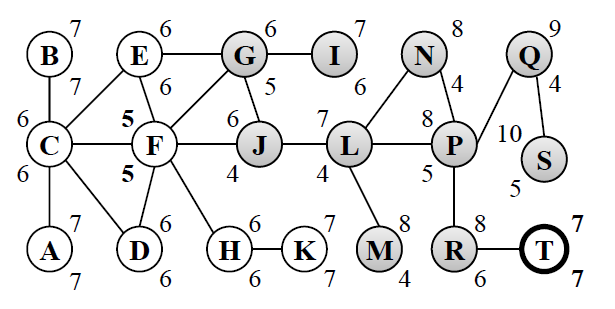
\includegraphics[scale=0.5]{image/graph.png}
\end{figure}
\newline Ici par exemple on peut supprimer soit le noeud A soit le noeud B.
\section{Implementation}
%% In this section we'll go over the most important parts of the code. As intructed
%% we have used the igraph library, and for the language we have chosen C++.\par
%% The function implementing the bounding eccentricity algorithm is the one with
%% the following signature:
Dans cette section, nous allons passer en revue les parties les plus importantes
du code. Comme indiqué, nous avons utilisé la bibliothèque igraph, et pour le
langage, nous avons choisi C++.\par La fonction qui implémente l'algorithme
Bounding Eccentricities est celle qui a la signature suivante :
i\begin{minted}{c++}
  void
  boundingEccentricities(const igraph_t& originalGraph,
                         std::vector<long>& eccentricities);
\end{minted}
%% Located in the eccentiricity.cc file. The structure of the function is what is
%% to be expected for an implementation of the bounding eccentricities algorithm.
%% And so we will rather focus more one the elements of the function that are not
%% as extensively detailed in the research paper. Thus we will mostly talk about
%% the candidate selection and graph prunning functions. \par
Situé dans le fichier eccentiricity.cc. La structure de la fonction est celle
que l'on peut attendre d'une implémentation de l'algorithme de Bounding
Eccentricity. Nous allons donc nous concentrer sur les éléments de la fonction
qui ne sont pas aussi détaillés dans l'article de recherche. Ainsi, nous
parlerons principalement des fonctions de sélection des candidats et pruning
du graphe. \par
\subsection{Sélection des candidats}
%% For the candidate selection function we have choosen the same approach chosen by
%% Frank Takes in his implementation of the Bounding Diameter algorithm located in
%% the following github repository:
%% \url{https://github.com/franktakes/teexgraph}. The candidate selection strategy
%% used in his code is the one nicknamed Interchanging eccentricity bounds. As
%% explained in the research paper this one consists in interchangeably selection
%% vertices with the highest and lowest eccentricity bounds each iteration. The
%% code responsible for keeping track of the lowest bound vertex is the follwoing
%% (as you can imagine the the one for the upper bound vertex is almost
%% identical):\newpage
Pour la fonction de sélection des candidats, nous avons choisi la même approche
que celle choisie par Frank Takes dans son implémentation de l'algorithme
Bounding Diameter situé dans le repo github suivant :
\url{https://github.com/franktakes/teexgraph}. La stratégie de sélection des
candidats utilisée dans son code est celle surnommée Interchanging eccentricity
bounds. Comme expliqué dans l'article de recherche, celle-ci consiste à
sélectionner de manière interchangeable les sommets ayant les limites
d'excentricité les plus élevées et les plus basses à chaque itération. Le code
responsable du suivi du sommet à la limite inférieure est le suivant (comme vous
pouvez l'imaginer, celui du sommet à la limite supérieure est presque
identique):\newpage
\begin{minted}{c++}
if (minLowerVertex == -1) {
  minLowerVertex = candidate;
} else if (lowerBounds[candidate] == lowerBounds[minLowerVertex] &&
           VECTOR(degrees)[candidate] > VECTOR(degrees)[minLowerVertex]) {
  minLowerVertex = candidate;
} else if (lowerBounds[candidate] < lowerBounds[minLowerVertex]) {
  minLowerVertex = candidate;
}
\end{minted}
%% These if/else clauses are run for every candidate in the candidate vector every
%% iteration. The first clause gets executed once every iteration and it's purpose
%% is essentially to allow the indexing of the \texttt{lowerBounds} vector in later
%% executions with other candidates. And finally, the second and third clauses
%% essentially store the candidate with minimal lower bound, and highest degree
%% case of lower bound equality in the \texttt{minLowerVertex} variable.  This
%% variable is then used at the start of each iteration in the
%% \texttt{selectCandidate} function of signature:
Ces clauses if/else sont exécutées pour chaque candidat du vecteur de candidats
à chaque itération. La première clause est exécutée une fois par itération et
son but est essentiellement de permettre l'indexation du vecteur
\texttt{lowerBounds} dans les exécutions ultérieures avec d'autres
candidats. Enfin, les deuxième et troisième clauses stockent essentiellement le
candidat ayant la borne inférieure minimale, et le degré le plus élevé en cas
d'égalité des bornes inférieures, dans la variable \texttt{minLowerVertex}.
Cette variable est ensuite utilisée au début de chaque itération dans la
fonction \texttt{selectCandidate} de signature:
\begin{minted}{c++}
long
selectCandidate(const std::set<long>& candidates,
                const long& minLowerVertex,
                const long& maxUpperVertex,
                bool& chooseUpper)
\end{minted}
%% which return the chosen candidate for the iteration.
qui renvoie le candidat choisi pour l'itération.
\subsection{Pruning}
%% The pruning strategy proposed in the paper, and thus implemented here, is about
%% removing all vertices of degree equal to one from the graph, and thus the
%% candidate vector, and setting their eccentricity to the eccentricity of the
%% single neighbor plus one after the main loop has finished executing. The
%% function responsible for this is:
La stratégie pruning proposée dans l'article, et donc mise en œuvre ici,
consiste à supprimer tous les sommets de degré égal à un du graphe, et donc du
vecteur candidat, et à fixer leur excentricité à l'excentricité du voisin unique
plus un après la fin de l'exécution de la boucle principale. La fonction
responsable de ceci est :
\begin{minted}{c++}
void
pruneGraph(igraph_t& graph,
           std::map<long, std::vector<long>>& prunedNeighborBuckets,
           long& prunedVertexCount) {
  bucketOutliers(graph, prunedNeighborBuckets);
  removeOutliers(graph, prunedNeighborBuckets, prunedVertexCount);
}
\end{minted}
%% The function in line 5 finds all vertices to be pruned and stores them in the
%% \texttt{prunedNeighborBuckets} map, which stores them the pruned vertices by
%% neighborhood, where the keys are the neighboors of the pruned vertices. The
%% following line 6 removes all of the previous vertices from the graph. \par
%% After all of the eccentricities of the vertices in the pruned graph have been
%% computed the following function is executed:
La fonction de la ligne 5 trouve tous les sommets à pruner et les stocke dans la
map \texttt{prunedNeighborBuckets}, qui stocke les sommets pruner par voisinage,
où les clés sont les voisins des sommets pruner. La ligne 6 suivante supprime
tous les sommets précédents du graphe. \par Après avoir calculé toutes les
excentricités des sommets du graphe pruner, la fonction suivante est exécutée :
\newpage
\begin{minted}{c++}
void
computePrunedEccentricities(
    const std::map<long, std::vector<long>>& prunedNeighborBuckets,
    std::vector<long>& eccentricities) {

  for (const auto& p : prunedNeighborBuckets) {
    long neighbor = p.first;
    const std::vector<long>& bucket = p.second;
    for (const auto& vertex : bucket) {
      eccentricities[vertex] = eccentricities[neighbor] + 1;
    }
  }
}
\end{minted}
Dans celle-ci, la variable \texttt{prunedNeighborBucket} est utilisée pour
calculer les excentricités des sommets pruner. Ceci est fait dans la ligne 10.
\section{Experiments}
%% In this section we present some performance analysis of our implementation of
%% this algorithm. To assess the performance of our implementation with respect to
%% the results found in section 6 of the paper [1] we provide some of the same
%% performance measures. We have thus measured the number of execution of our
%% shortest path search algorithm required to compute all of the eccentricities. In
%% this section we shall first analyse the performance of the different selection
%% strategies as well as the graph prunning strategy given in the paper. The number
%% of iteration taken after the implementation of each method presented in the
%% respective columns for the ca-CondMat, ca-HepPh and ca-HepTh is given in the
%% following table:
Dans cette section, nous présentons une analyse des performances de notre
implémentation de cet algorithme. Pour évaluer les performances de notre
implémentation par rapport aux résultats trouvés dans la section 6 de l'article
[1], nous fournissons certaines des mêmes mesures de performance. Nous avons
ainsi mesuré le nombre d'exécution de notre algorithme de recherche du plus
court chemin nécessaire pour calculer toutes les excentricités. Dans cette
section, nous allons d'abord analyser les performances des différentes
stratégies de sélection ainsi que la stratégie de prunning du graphe donnée dans
l'article. Le nombre d'itérations prises après l'implémentation de chaque
méthode présentée dans les colonnes respectives pour les ca-CondMat, ca-HepPh et
ca-HepTh est donné dans le tableau suivant :\\
\begin{center}
 \begin{tabular}{||c c c c c||} 
   \hline
   Dataset & Random & Pruning & Interchanging bound & Degree centrality \\
   \hline\hline
   ca-HepPh & 8444 & 8211 & 1662 & 1589 \\
   \hline
   ca-HepTh & 6175 & 5886 & 1101 & 1053 \\
   \hline
   ca-CondMat & 9439 & 9268 & 3486 & 3271 \\ 
   \hline
 \end{tabular}
\end{center}
\medskip
\noindent
The best performing variant was evaluated on 2 more datasets of higher
sizes. The following table shows the results:\\
\begin{center}
 \begin{tabular}{||c c c c c||} 
   \hline
   Dataset & Nodes & Edges & Pruned & Iterations \\
   \hline\hline
   ca-HepPh & 11\ 204 & 117\ 619 & 282 & 1\ 589 \\
   \hline
   ca-HepTh & 8\ 638 & 24\ 806 & 351 & 1\ 051 \\
   \hline
   ca-CondMat & 21\ 363 & 91\ 286 & 353 & 3\ 271 \\ 
   \hline
   web-NotreDame & 325\ 729 & 1\ 090\ 108 & 141\ 178 & 142 \\
   \hline
   web-Stanford & 255\ 265 & 1\ 941\ 926 & 1\ 0350 & 9 \\
   \hline
 \end{tabular}
\end{center}
\section{Conclusion}
%% We have thus implemented the algorithm and have found very similar results for
%% each of the graphs used in the paper. We also have seen the relative improvement
%% of each optimization method proposed in the paper. However, there are still some
%% improvements that can be performed. A possible route for improvement would be to
%% find a better candidate selection method, however this would require more
%% research to be performed. Another route for improvement that would require less
%% effort would be to parallelise the shortest path computations to leverage as
%% most as possible multiple core systems which are much more popular today than
%% they were in 2013.
Nous avons donc implémenté l'algorithme et avons trouvé des résultats très
similaires pour chacun des graphes utilisés dans l'article. Nous avons également
constaté l'amélioration relative de chaque méthode d'optimisation proposée dans
l'article. Cependant, certaines améliorations peuvent encore être réalisées. Une
voie d'amélioration possible serait de trouver une meilleure méthode de
sélection des candidats, mais cela nécessiterait plus de recherches. Une autre
voie d'amélioration qui demanderait moins d'efforts serait de paralléliser les
calculs du plus court chemin afin d'exploiter au maximum les systèmes à
plusieurs cœurs qui sont beaucoup plus populaires aujourd'hui qu'ils ne
l'étaient en 2013.
\section{References}
\begin{enumerate}
\item Takes, F.W.; Kosters, W.A. Computing the Eccentricity Distribution of Large Graphs. Algorithms 2013, 6, 100-118. https://doi.org/10.3390/a6010100
\item Frank W. Takes and Walter A. Kosters. 2011. Determining the diameter of small world networks. In Proceedings of the 20th ACM international conference on Information and knowledge management (CIKM '11). Association for Computing Machinery, New York, NY, USA, 1191–1196. DOI:https://doi.org/10.1145/2063576.2063748
\end{enumerate}
\end{document}
